\chapter{Developer Manual}
\label{appendix-developer-manual}
This manual will go through the needed steps to get started on extending and further developing on OKSE. The first sections will go through how to set up the development environment. The rest of the sections will go through the different parts of the system and how you can extend them.

\section{Requirements and Setup}
The recommended setup, as noted below, is using IntelliJ IDEA\footnote{\url{https://www.jetbrains.com/idea/}} as the Java IDE. However, other IDEs that meet the requirements listed below, or a combination should suffice. 

\subsection{Requirements and dependencies}

\subsubsection{Java}
The minimum required major version of Java is 8, and we do recommend to use the latest minor release. As of the writing of this guide, update 31 is the latest, and the version which is used to compile the packaged version of OKSE that is bundled.

\subsubsection{Apache Maven}
The project source code, tests and dependency management is structured with Apache Maven\footnote{\url{https://maven.apache.org}}. Maven is used to fetch dependencies, run the tests and to build the final jar files. The minimum major version of Maven is 3 and any minor version from 3.0.5 and up can be used. However, the development team recommends the latest version. As of the time of this writing, the latest version is 3.3.3.

It is worth mentioning, that many of the popular IDE software for Java bundles Maven support and does not require it to be installed separately on the system.

\subsection{Recommended IDE}
The development team strongly recommends IntelliJ IDEA Ultimate\footnote{\url{https://www.jetbrains.com/idea/}} as the Integrated Development Environment. Note that the free Community edition should suffice, but its worth mentioning that the Ultimate edition has better support for frameworks like Spring and TestNG (test framework of choice), which is used for the web administration interface. Both Community and Ultimate edition comes bundled with Maven.

\subsection{Test Framework: TestNG}
The system has a lot of unit tests, and the test framework of choice is TestNG\footnote{\url{http://testng.org/doc/index.html}}. Any new features and expansions of the system should be accompanied by unit tests. Please refer to the TestNG documentation\footnote{\url{http://testng.org/doc/documentation-main.html}} on how to write tests that suits the expansions needs.

\subsection{IntelliJ setup}
As the user stands free to choose the IDE, the setup documentation will be fairly basic and it will be based on IntelliJ.

Prerequisites: IntelliJ is installed, an Internet connection and the source code is stored locally.

\begin{enumerate}
\setlength{\itemsep}{0cm}%
    \item Open IntelliJ
    \item Click "Import Project" or File -> "Import Project"
    \item Browse the file system and select the source code folder
    \item Choose "Import project from external model"
    \item Choose "Maven"
    \item Check "Import Maven projects automatically"
    \item Click Next
    \item no.ntnu.okse... should be selected, click Next
    \item Select 1.8 (if it is not available, click "+" and add it)
    \item Click Next
    \item Click Finish
\end{enumerate}

After the IntelliJ window is opened with the project, all the needed dependencies will be downloaded. After this is complete, the project setup is complete.

\section{Overview of components}

\subsection{Application}

The \verb!Application.java! file that resides in the root of the project is the main invocation point when starting the OKSE application. The main operations performed in this class are initializing the web admin console, and the CoreService instance, which in turn boot up more services.

The most important thing to note regarding this main class, is that it is also the class in which further extensions should be registered. Extending the application with additional core services is done through registering them to the CoreService via the \verb!registerCoreService()! method.

Extending the application with additional protocol support is done through use of the \verb!addProtocolServers()! method of the CoreService instance.

\subsection{Web Admin}

The OKSE administration console is run using the Spring framework, more exact the spring-boot package\footnote{\url{https://spring.io/guides/gs/rest-service/}}, using Thymeleaf-templates\footnote{\url{http://www.thymeleaf.org}}. The main aspects of the Web Admin component are its models, controllers, templates and front-end JavaScript. The administration interface of OKSE is built in a modular way, to achieve loose coupling. Each pane of the interface has its own controller and respectively a front-end JavaScript.  With this approach it's easy to extend the web interface.

\subsubsection{Back-end}

The back-end of OKSE works as a RESTful Web Service. It's responsible for working as a link between the administration interface and all the different registered services in OKSE. Since the back-end uses the Spring framework, the main architectural approach for the back-end is based upon Spring’s approach for building RESTful web services. All HTTP-requests are handled by a dedicated controller. These controllers are easily identified by the \verb!@RestController! annotation. Each controller are responsible for handling all HTTP-requests defined by \verb!@RequestMapping! annotations.  

\subsubsection{Front-end}

The front-end of OKSE is the only component of the system directly accessible for user interaction. It's responsible for making HTTP-requests to the back-end for manipulation and presentation of the state OKSE is in. To ensure and minimize the probability for cross-browser incompatibilities, the front-end is implemented using jQuery. Each pane of the administration interface has its own module implemented with jQuery. Each of this modules are responsible for event-handling, AJAX-requests and DOM-manipulation in its own pane.

\subsection{CoreService}

The CoreService is the main part of the OKSE message translation and brokering system. It is responsible for booting and stopping the registered core services, such as those described in subsequent sections of this manual.

Additionally, the CoreService boots up registered ProtocolServers, which are described in their own section below. The CoreService is also responsible for gracefully shutting down registered ProtocolServers.

As with all the OKSE core services, the main CoreService extends the AbstractCoreService class. This class holds some common attributes that are needed, as well as definitions of the abstract methods for \verb!init()!, \verb!boot()!, \verb!run()! and \verb!stop()! actions.

All the services are intended to follow the singleton pattern, which in our implementation uses static references. Thus, the remaining needed methods and fields for initialization and instantiation are not provided by the abstract super class. They have to be implemented using a similar approach as described in the \ref{sec:common-patterns-used} and \ref{sec:adding-new-core-services} chapters.

An overview of the boot sequence of the main OKSE components is described in figure \ref{fig:boot-sequence}.


\begin{center}
  \begin{figure}[ht!]
    \makebox[\textwidth]{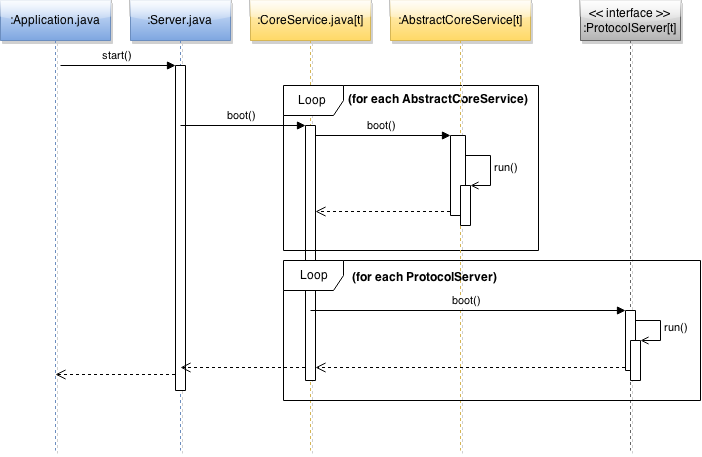
\includegraphics[width=\textwidth]{fig/bootSequence.png}}
    \caption{Boot sequence main components of OKSE}
    \label{fig:boot-sequence}
  \end{figure}
\end{center}

The details of the \verb!init()!, \verb!boot()! and \verb!run()! methods will vary from service to service, and protocol server to protocol server.

After the boot sequence has completed, all of the instances of either core services or protocol servers have their own dedicated thread that awaits the next task or event to execute.

\subsection{TopicService}

\subsection{SubscriptionService}

\subsection{MessageService}

\subsection{ProtocolServer}
 
\subsubsection{WSNotificationServer}

\subsubsection{AMQPServer}

\section{Common Patterns Used}
\label{sec:common-patterns-used}

\begin{itemize}
\item Singelton
\item ObserverPattern
\item Other: \begin{itemize}
\item Event Driven Single Service Single Thread
\end{itemize}
\end{itemize}

\section{Adding new protocols}

Something about AbstractProtocolServer class and ProtocolServer interface

\section{Adding new core services}
\label{sec:adding-new-core-services}

Something about AbstractCoreService, Singleton pattern and the needed methods to accomplish this, and the abstract methods needed from the super class

\section{Extending the administration interface}
\label{sec:adding-new-panes}

\begin{center}
  \begin{figure}[ht!]
    \makebox[\textwidth]{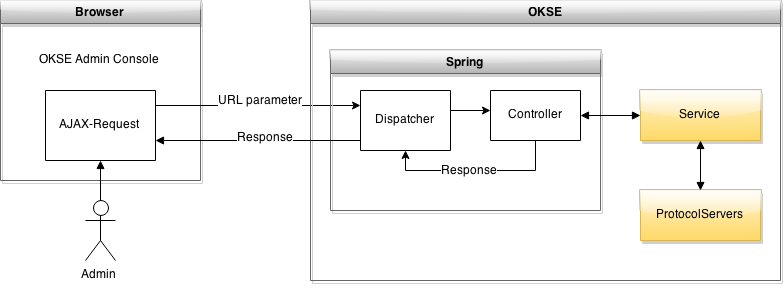
\includegraphics[width=\textwidth]{fig/oacRequestFlow.png}}
    \caption{Request flow for the administration panel}
    \label{fig:oac-request-flow}
  \end{figure}
\end{center}

This section describes how to create or extend the administration interface with new content and functionality. The modularity of the administration interface makes this easy. Figure \ref{fig:oac-request-flow} visualises how the OKSE system handles events and exposes information to the users. The key concepts to notice here is the AJAX-requests and the controllers. On an event, whether it is a page auto update or a button-click, the request URL is accessed by the AJAX-request. Spring's dispatcher maps the URL and forwards it to the correct controller. This controller interacts with OKSE's services and returns a response.

As of the time of this writing, OKSE contains of seven JavaScript modules: 

\begin{description}
    \item[main.js] \hfill \\ Responsible for the "Main"-pane. This module also contains all logic for setting the update interval for all the other panes. Also this is the location of the AJAX-module. 
    \item[topics.js] \hfill \\ Responsible for the "Topics"-pane. This module contains all logic regarding topics, which includes, but are not limited to, refreshing the table containing all topics. 
    \item[subscribers.js] \hfill \\ Responsible for the "Subscribers"-pane. This module contains all logic regarding subscribers, which includes, but are not limited to, refreshing the table containing all subscribers. 
    \item[stats.js] \hfill \\ Responsible for the "Statistics"-pane. This module contains all logic for refreshing the statistics from OKSE.
    \item[logs.js] \hfill \\ Responsible for the "Logs"-pane. This module requests the given log from OKSE and visualizes it.
    \item[config.js] \hfill \\ Responsible for the "Configuration"-pane. This module is responsible for configuration OKSE. This includes for instance the possibility to add topic mappings. 
    \item[paginator.js] \hfill \\ This module controls all logic regarding the paginator that appear when the topic/subscriber tables exceed 25 elements. 
    \item[okseDebug.js] \hfill \\ This is a jQuery-plugin that appends a logger to the document.
\end{description}

Hopefully, after reading this introduction you have gotten a fair understanding of how the administration interface is structured. The following steps will explain how to actually extend the application. In addtition, if you are completely new to Thymeleaf-templates, Spring framework or jQuery/Javascript, it would be a good idea to check out the following resources: 

\begin{itemize}
\setlength{\itemsep}{0cm}%
\item Thymeleaf - see \url{http://www.thymeleaf.org/documentation.html}
\item Spring framework - see \url{https://spring.io/guides/gs/rest-service/}
\item jQuery - see \url{http://jqfundamentals.com}
\item JavaScript - see \url{https://developer.mozilla.org/en-US/docs/Web/JavaScript/A_re-introduction_to_JavaScript}
\end{itemize}

\subsection{Administration interface structure}

All files for the administration interface are located in three main folders, \verb!static/js!, \verb!templates! and \verb!web!. See figure \ref{fig:oac-folder-hierarchy} for a detailed overview. To extend the application you can just copy and modify existing files, or create new ones based on the skeleton provided in section \ref{subsubsec:skeletons}. The files needed to be modified of created are:

\begin{itemize}
\item HTML template files in \verb!src/resources/templates/!
\item JavaScript files in \verb!src/resources/static/js/!
\item Spring controllers in \verb!src/no/ntnu/okse/web/controller/! 
\end{itemize}

\begin{center}
  \begin{figure}[ht!]
    \makebox[\textwidth]{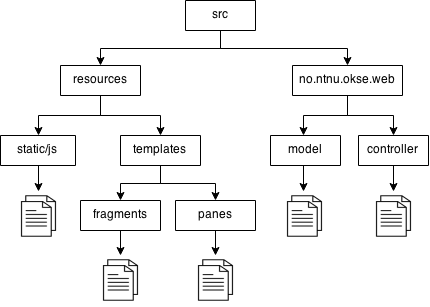
\includegraphics[scale=0.4]{fig/oacFolders.png}}
    \caption{Folder hierarchy for the administration interface}
    \label{fig:oac-folder-hierarchy}
  \end{figure}
\end{center}



\subsubsection{Skeletons}
\label{subsubsec:skeletons}

Below is a skeleton for adding a new REST controller. The same applies for normal controllers, but then the \verb!@Controller! annotation is used in stead of the \verb!@RestController! annotation. When using this annotation, Spring will automatically find the controller on boot, and add the mapping to the dispatcher. 

\begin{lstlisting}[language=Java, captionpos=b, caption=Skeleton for a REST-controller, frame=bt, showstringspaces=false]
@RestController
@RequestMapping(value = "/api/MYPANE") // Base URL
public class TestController() {
    
    private static final String TEST_URL = "/get/all";
    
    @RequestMapping(value = TEST_URL, method = RequestMethod.GET)
    public @ResponseBody void getAllInfo() {
        return "This is a test";
    }
    
}
\end{lstlisting}

Below is a skeleton for adding a new JavaScript module on the web page for displaying information from a controller. This only shows briefly how one would start to create new modules. To add the JS-file to the administration interface on rendering, append \verb!<script th:src="/js/<MODULE>.js"></script>! to the \verb!th:block! identified with "scripts" in the \verb!indexLoggedIn.html! template. \\ 

\begin{lstlisting}[language=Java, captionpos=b, caption=Skeleton for a JavaScript module, frame=bt, showstringspaces=false]
var MYPANE = (function($) { 

    var initateModule = function() {
    
    }

    return {
        init = intiateModule
    }

})(jQuery)
\end{lstlisting}

\begin{lstlisting}[language=HTML, captionpos=b, caption=Skeleton for a Thymeleaf-template, frame=bt, showstringspaces=false]
<html xmlns:th="http://www.thymeleaf.org"
      xmlns:layout="http://www.ultraq.net.nz/web/thymeleaf/
      layout"
      xmlns:sec="http://www.thymeleaf.org/thymeleaf-extras
      -springsecurity3"
      layout:decorator="layout">
<head>
</head>
<body>
<th:block layout:fragment="MYPANE">
<div class="tab-pane" id="MYPANE">
...
</div>
</th:block>
</body>
</html>
\end{lstlisting}

If you choose to add a new pane it's important to register the panes JavaScript module in the \verb!main.js! file. This is done by appending a \verb!switch-case! for your pane. Also remember to register the panes template in \verb!indexLoggedIn.html!

\section{AMQP Send and Receive}

\clearpage